\documentclass{beamer}

%%%%%% PACKAGES %%%%%%
\usepackage[utf8x]{inputenc}
\usepackage[T1]{fontenc}
\usepackage[english]{babel}

\usepackage{hyperref}
\usepackage[numbers]{natbib}
\usepackage{array}
\usepackage{graphicx}
\usepackage{tikz}
\usetikzlibrary{snakes,arrows,shapes,calc}

%%%%%%%%%% CUSTOM COMMANDS %%%%%%%%%%

\newcommand{\okay}{
\includegraphics[height=0.5cm]{img/check.png}}
\newcommand{\nope}{
\includegraphics[height=0.5cm]{img/cross.png}}
\newcommand{\sortof}{
\includegraphics[width=0.5cm]{img/tilde.png}}

\newcommand{\ZZ}{\mathbb{Z}}
\newcommand{\Uu}{\mathcal{U}}

\newcommand{\la}{\leftarrow}
\newcommand{\ra}{\rightarrow}
\newcommand{\lra}{\leftrightarrow}

\newcommand{\Lla}{\longleftarrow}
\newcommand{\Lra}{\longrightarrow}
\newcommand{\Llra}{\longleftrightarrow}

\newcommand{\set}[1]{\left\{ #1 \right\}}


%%%%%%%% THEME %%%%%%%%
\usetheme[sectionpage=progressbar, progressbar=frametitle, block=fill]{metropolis}

%%%%%%% METADATA %%%%%%%
\title{Secure Group Messaging}
\author{Simon Fernandez}
\date{\today}


%%%%%%%%%%%%%%%%%%%%%%%%%%%
%%%%%%%%%% START %%%%%%%%%%
\begin{document}

\maketitle

\begin{frame}{Overview}
  \setcounter{tocdepth}{1}
	\tableofcontents
\end{frame}

\section{Group conversations ?}
\begin{frame}{Properties of real life and messaging conversations}
	\begin{tabular}{cc}
  	\begin{tabular}{c}
    	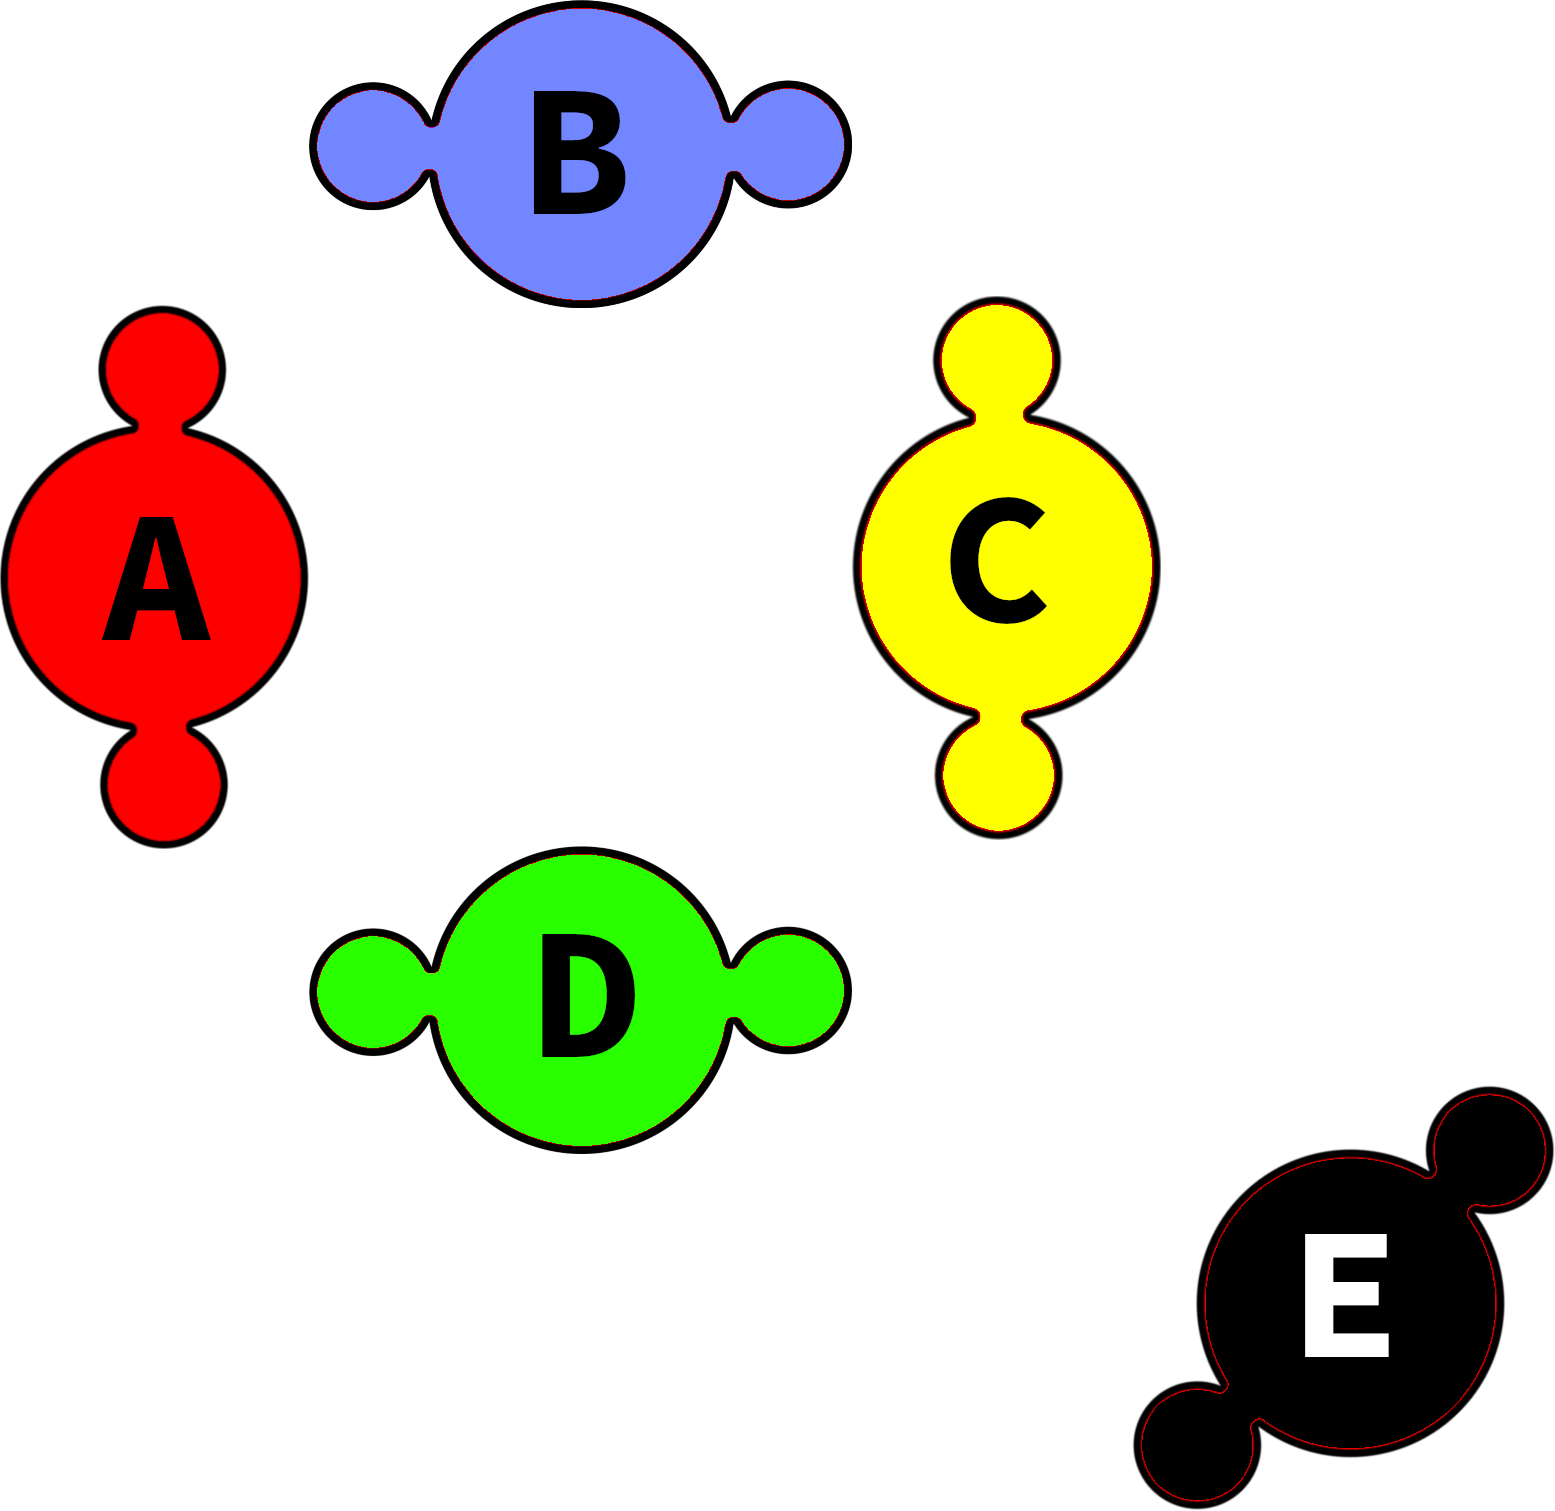
\includegraphics[height=5cm]{img/group_chat_eve.png}
  	\end{tabular} &

  	\begin{tabular}{c}
  		Authentification \\
  		\hline
  		Participants Coherence \\
  		Transcript Coherence \\
  		\hline
  		Message Repudiation \\
  		Participation Repudiation \\
  		\hline
  		Dynamic Groups \\
  		\hline
  		Forward Secrecy \\
  		Backward Secrecy \\
  		Non-Transitivity of Messages \\
  		\hline
  		Asynchrone
    \end{tabular}
	\end{tabular}
\end{frame}

\begin{frame}{Why is it harder than regular peer-to-peer?}
	\begin{tabular}{cc}
  	\begin{tabular}{c}
    	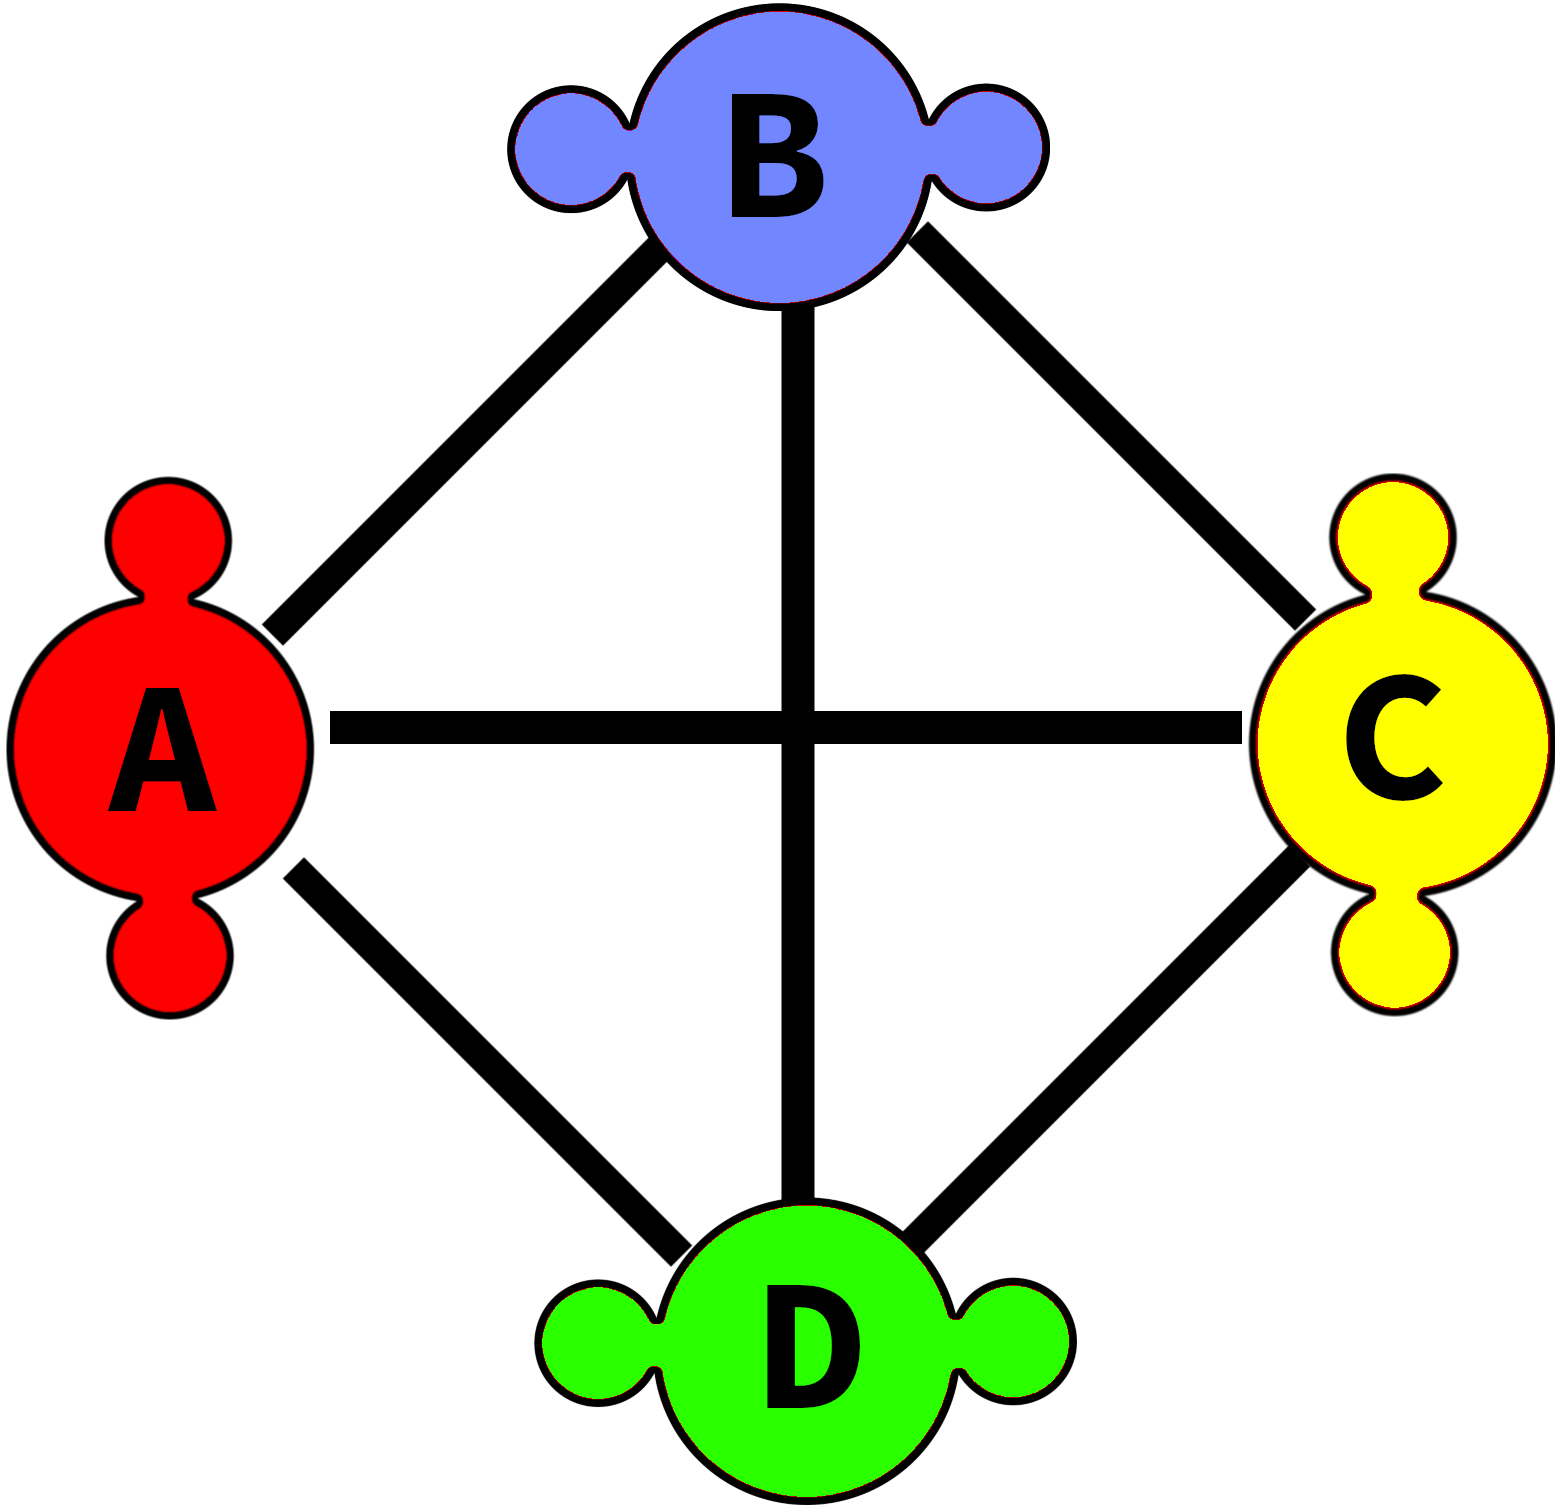
\includegraphics[height=5cm]{img/group_p2p.png}
  	\end{tabular} &

  	\begin{tabular}{c}
  		Participants Coherence \\
  		Transcript Coherence
    \end{tabular}
	\end{tabular}

\end{frame}


\section{mpOTR}
\begin{frame}{mpOTR – Ian Goldberg et al. 2009~\cite{mpotr}}
	\begin{block}{Initialisation}
		\begin{itemize}
			\item Agree on the list of participants
			\item Group key exchange
			\item Deduce the signature and cypher key
		\end{itemize}
  \end{block}

	\begin{block}{Communication}
		\begin{itemize}
			\item Sign the message
			\item Cypher with group key
			\item Broadcast to all
		\end{itemize}
  \end{block}

	\begin{block}{Shutdown}
		\begin{itemize}
			\item Agree on transcript
			\item Delete keys
		\end{itemize}
  \end{block}
\end{frame}

\begin{frame}{mpOTR}
	\center
  	\begin{tabular}{c|c}
			 & mpOTR \\
			\hline
  		Authentification & \okay \\
  		\hline
  		Participants Coherence & \okay \\
  		Transcript Coherence & \okay \\
  		\hline
  		Message Repudiation & \okay \\
  		Participation Repudiation & \okay \\
  		\hline
  		Dynamic Groups & \nope \\
  		\hline
  		Forward Secrecy & \nope \\
  		Backward Secrecy & \nope \\
  		Non-Transitivity of Messages & \nope \\
  		\hline
  		Asynchrone & \sortof 
    \end{tabular}
\end{frame}


\section{GOTR}
\begin{frame}{GOTR – Liu et al~\cite{gotr}}
	\center
	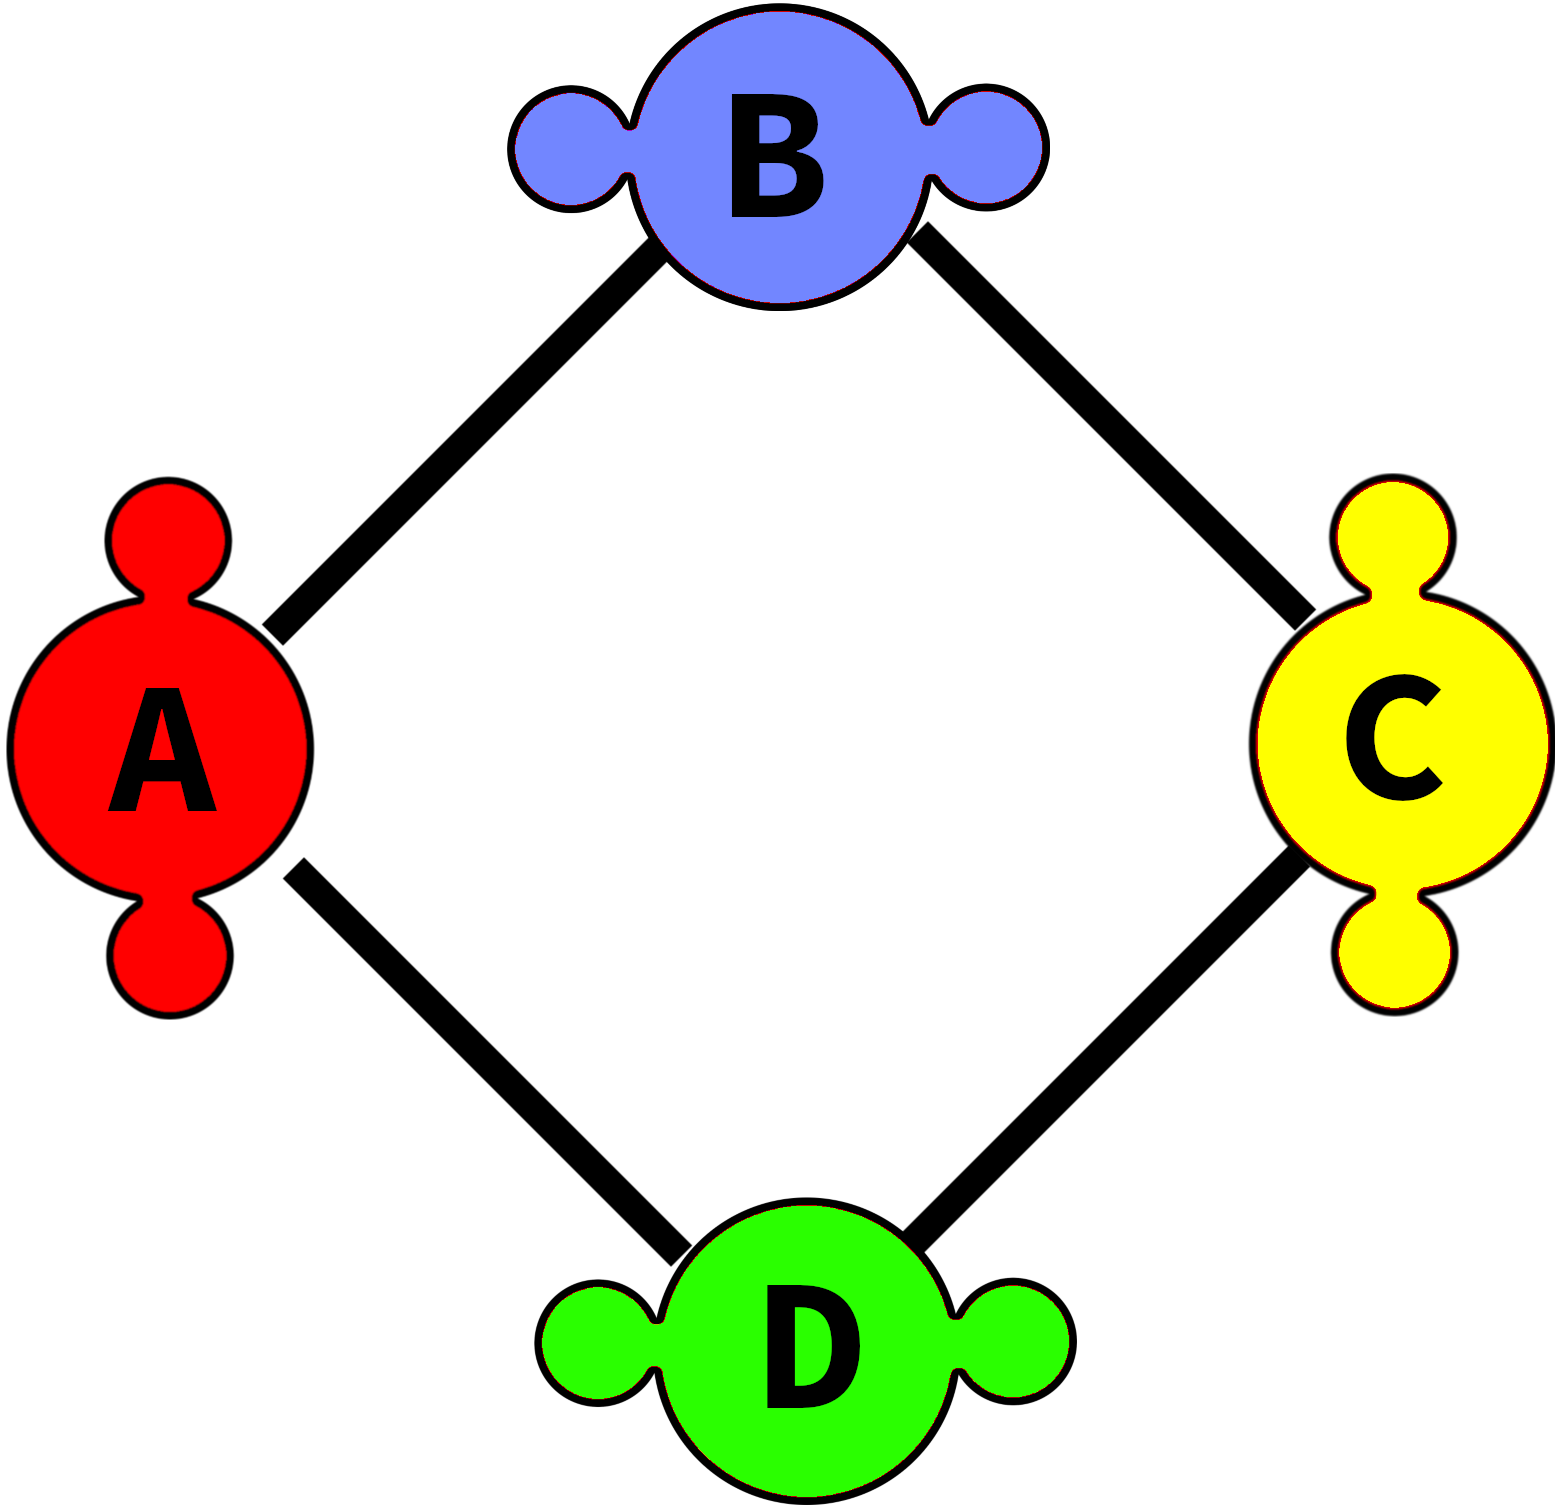
\includegraphics[height=6cm]{img/group_ring4.png}
\end{frame}

\begin{frame}{GOTR – Liu et al~\cite{gotr}}
	\center
	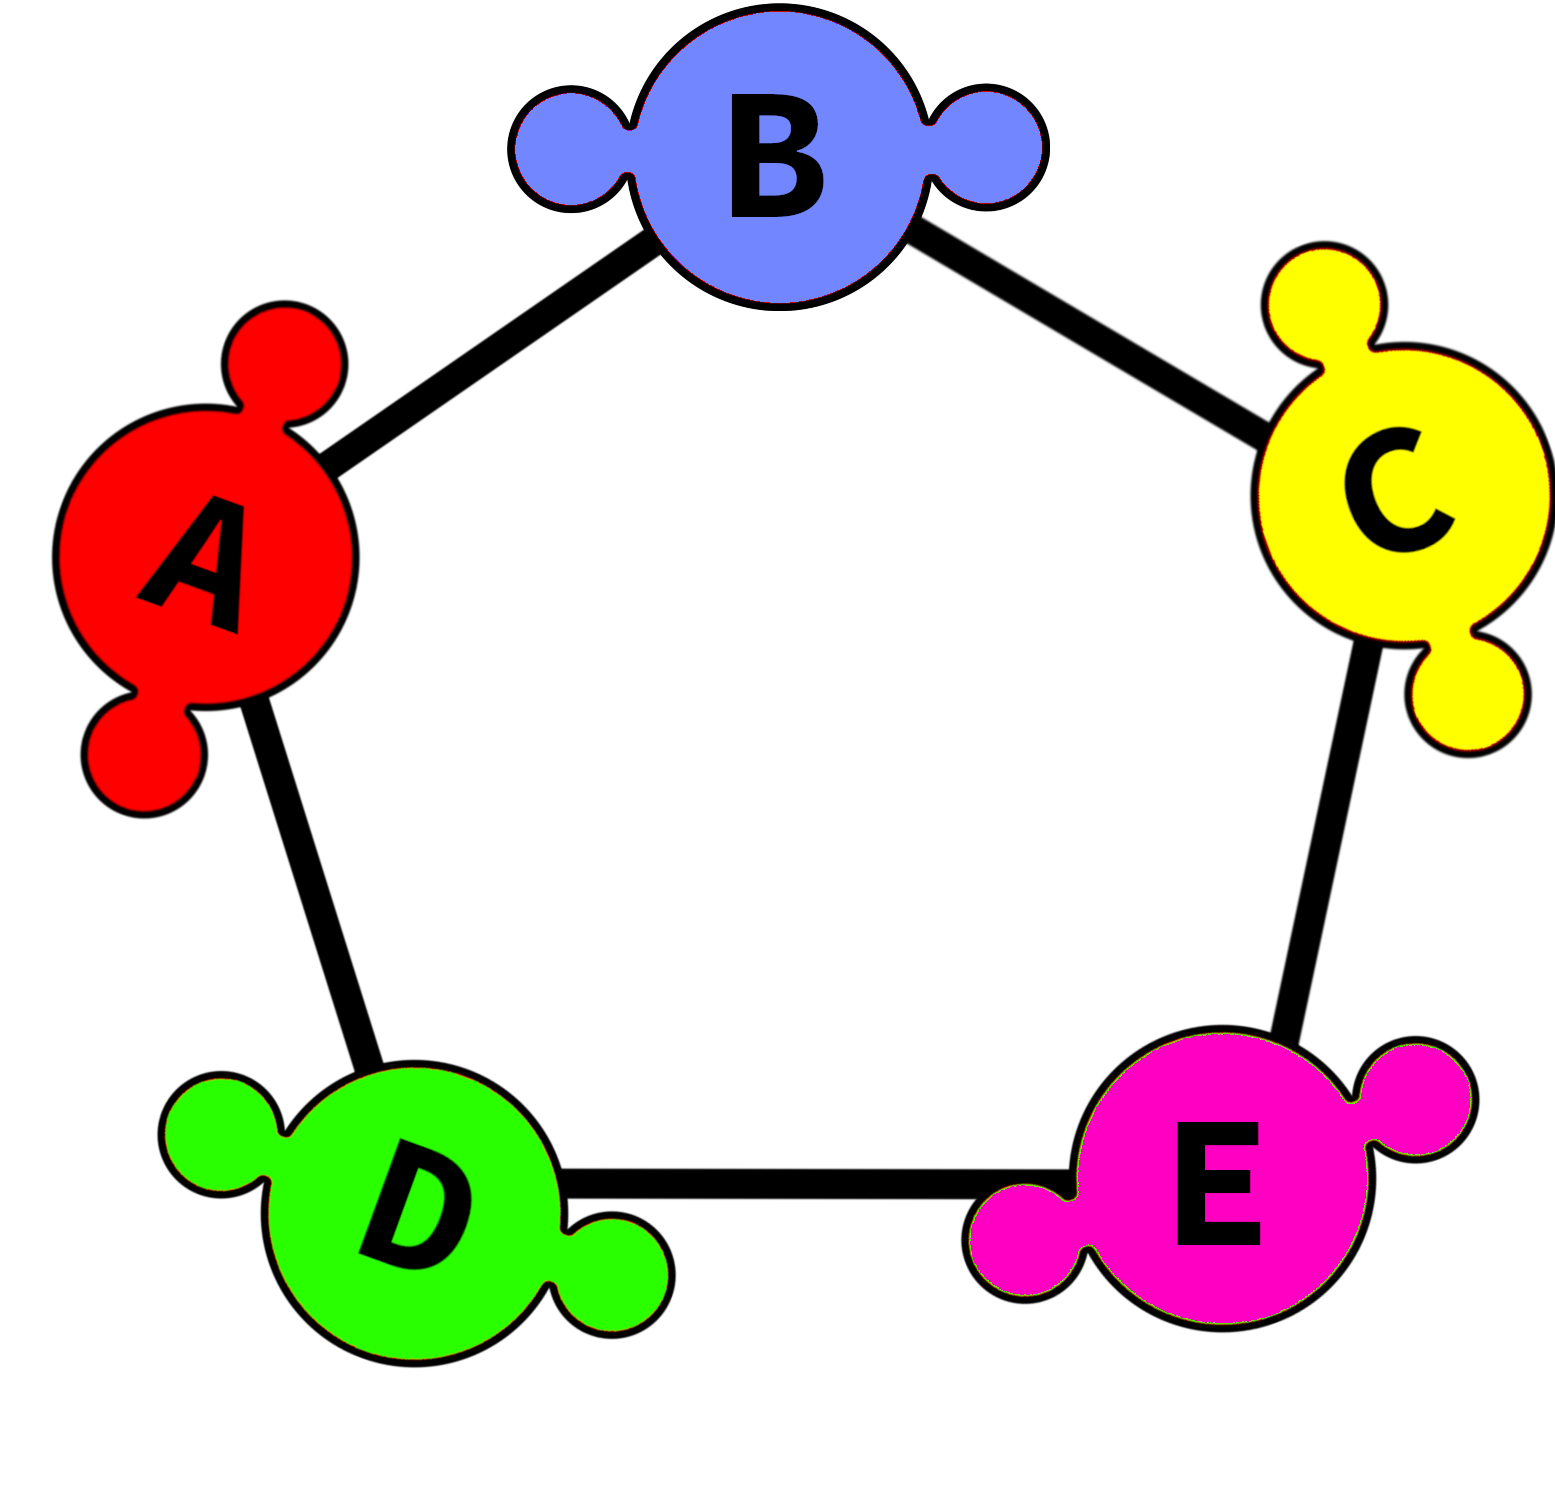
\includegraphics[height=6cm]{img/group_ring5.png}
\end{frame}

\begin{frame}{GOTR}

	\begin{block}{Update Key}
		\begin{itemize}
			\item Generate a new cypher and sign key
			\item Individual : consistency check
			\item Individual : send the new keys
			\item Deduce the new group key
		\end{itemize}
  \end{block}

	\begin{block}{Join/Part}
		\begin{itemize}
			\item Add to the circle
			\item Call the UpdateKey protocol
		\end{itemize}
  \end{block}
\end{frame}

\begin{frame}{GOTR}
	\center
  	\begin{tabular}{c|cc}
			 & mpOTR & GOTR\\
			\hline
  		Authentification & \okay & \okay \\
  		\hline
  		Participants Coherence & \okay & \okay \\
  		Transcript Coherence & \okay & \okay \\
  		\hline
  		Message Repudiation & \okay & \okay \\
  		Participation Repudiation & \okay & \okay \\
  		\hline
  		Dynamic Groups & \nope & \okay \\
  		\hline
  		Forward Secrecy & \nope & \sortof \\
  		Backward Secrecy & \nope & \sortof \\
  		Non-Transitivity of Messages & \nope & \okay \\
  		\hline
  		Asynchrone & \sortof & \nope 
    \end{tabular}
\end{frame}

\section{Signal}
\begin{frame}{Technical point : Diffie-Hellman}
	\center
	
\includegraphics[height=8cm]{img/stand-back-im-gonna-try-science.jpg} 
\end{frame}

\begin{frame}{Diffie-Hellman Key Exchange}
	\begin{block}{The Group}
		\begin{itemize}
			\item Cyclic Group $(G, \cdot)$ of prime order $p$
			\item $\forall g \in G, g^p = e_G, g^{(p+1)} = g$
			\item Let $g \in G\setminus \set{e_G}$. $\forall a \in G, \exists n \in \ZZ / p\ZZ, a = g^n$
		\end{itemize}
	\end{block}

	\pause

	\begin{block}{Exchange}
	$$
    \begin{array}{rl}
      A :& x \la \Uu(\ZZ / q\ZZ) \\
      B :& y \la \Uu(\ZZ / q\ZZ) \\
      A \ra B :& g^x \\
      B \ra A :& g^y \\
      A :& S = (g^y)^x \\
      B :& S = (g^x)^y \\
    \end{array}
   $$
	\end{block}

\end{frame}

\begin{frame}{Peer-to-peeer 1.0 : Diffie-Hellman Ratchet}
	\begin{block}{Initialisation}
		Do a DH key exchange : common secret $S_0 = g^{xy}$
	\end{block}

	\begin{block}{Communication}
	$$
      \begin{array}{rl}
        A :& x' \la \Uu(\ZZ / q\ZZ) \\
        A \ra B :& \set{M, g^{x'}}_{S_0} \\
        A :& S_1 = (g^y)^{x'} \\
        B :& S_1 = (g^{x'})^y \\
        B :& y' \la \Uu(\ZZ / q \ZZ) \\
        B \ra A :& \set{M', g^{y'}}_{S_1} \\
        B :& S_2 = (g^{x'})^{y'} \\
        A :& S_2 = (g^{y'})^{x'} \\
      \end{array}
      $$
	\end{block}
\end{frame}

\begin{frame}{Peer-to-peeer 2.0 : Diffie-Hellman Double Ratchet}
	\center
	\begin{tabular}{rcl}
		Alice & & Bob \\
		\hline
    $(x_0, g^{x_0})$ & $\Llra$ & $(y_0, g^{y_0})$ \\
		\hline
		$S_0$ & & $S_0$ \\
		\hline
		$\set{M_0, g^{x_1}}_{S_0}$ & $\Lra$ & \\
		\hline
		$S_{0, 1} \la H(S_0)$  & & \\
		\hline
		$\set{M_1, g^{x_1}}_{S_{0, 1}}$ & $\Lra$ & \\
		\hline
		$S_{0, 2} \la H(S_{0, 1})$  & & \\
		\hline
		$\set{M_2, g^{x_1}}_{S_{0, 2}}$ & $\Lra$ & \\
		\hline
		 & & $S_1 \la (g^{x_1})^{y_0}$ \\
		\hline
		 & $\Lla$ & $\set{M_3, g^{y_1}}_{S_1}$
	\end{tabular}
\end{frame}

\begin{frame}{Signal : Peer-to-peer DHDR}
	\center
	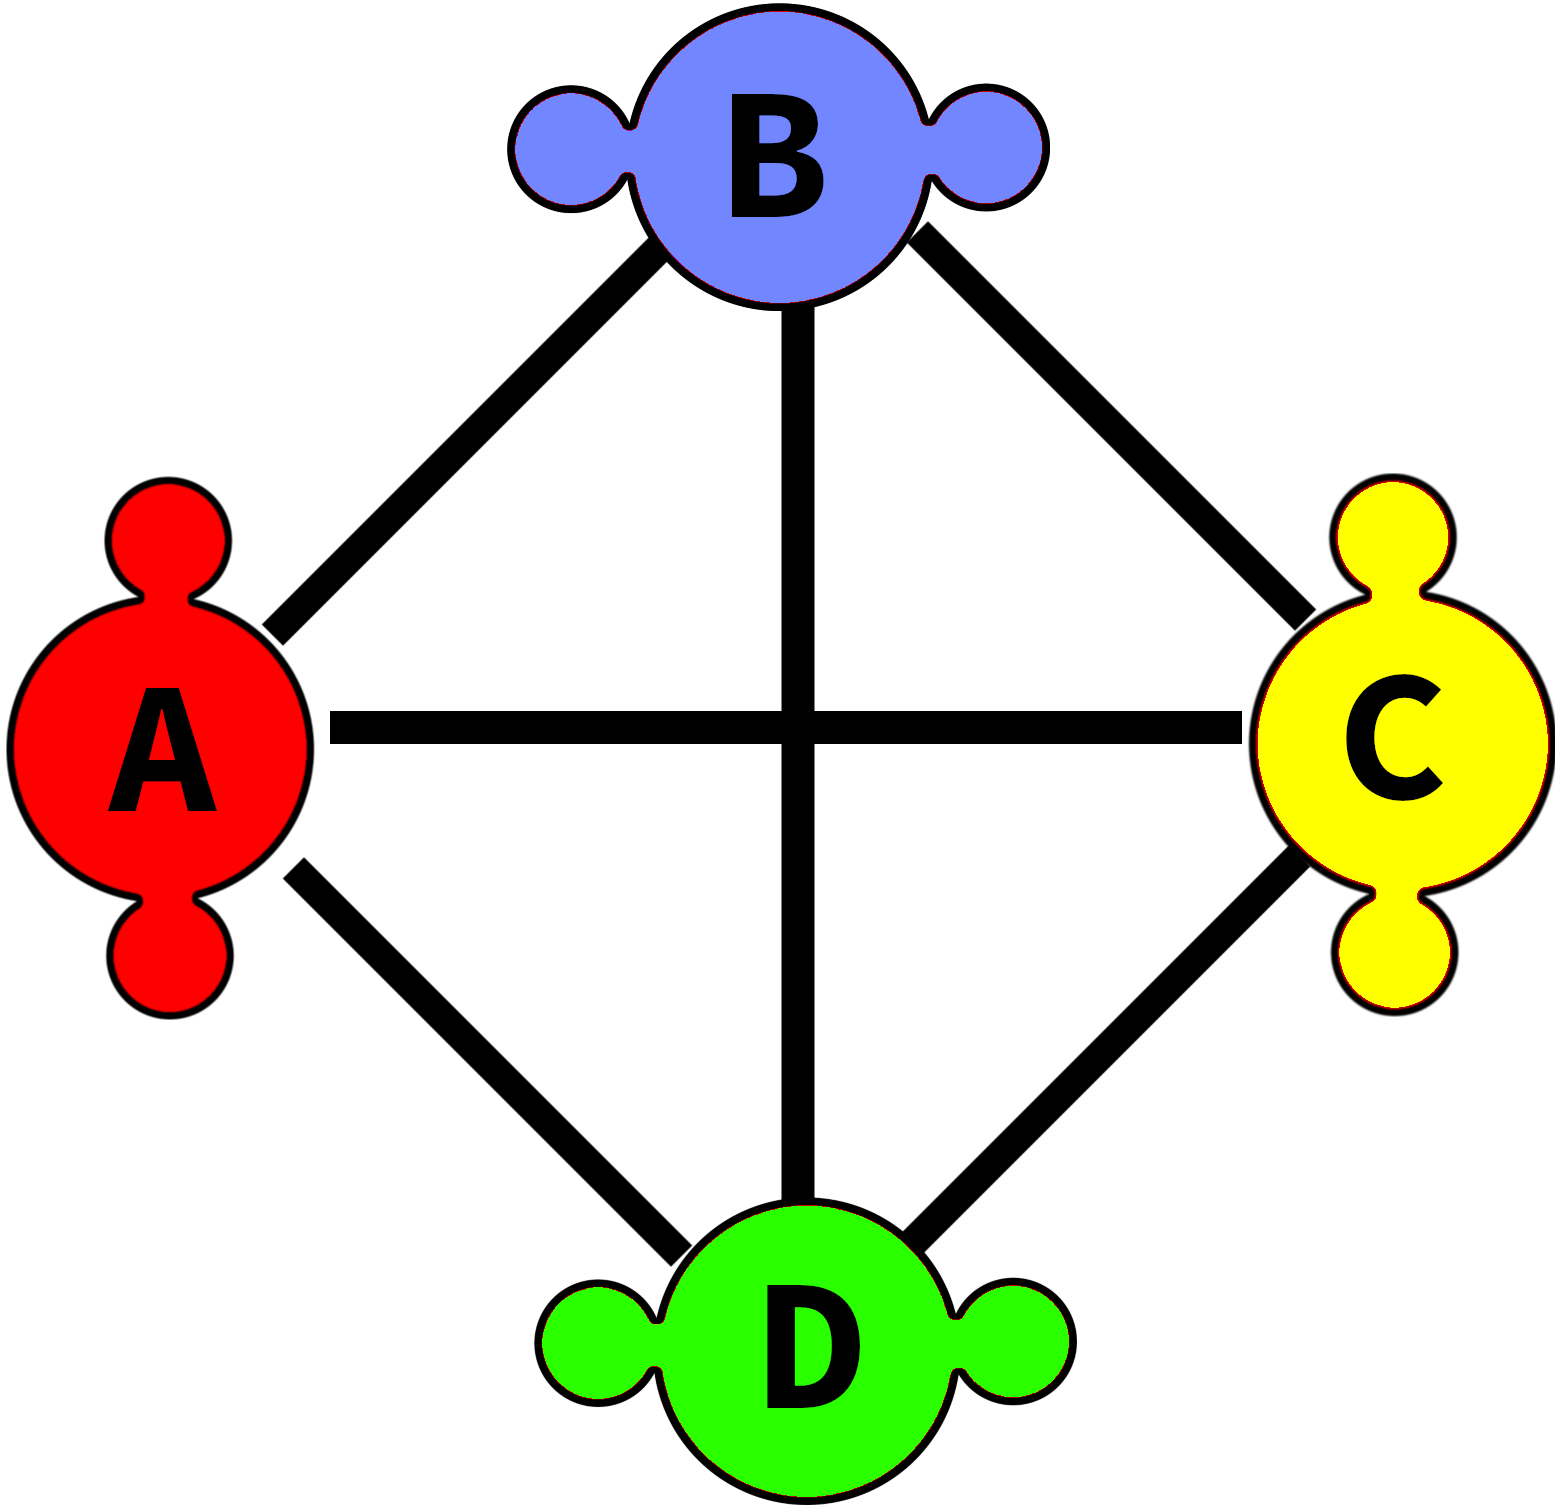
\includegraphics[height=6cm]{img/group_p2p.png}
\end{frame}

\begin{frame}{Signal}
	\center
  	\begin{tabular}{c|ccc}
			 & mpOTR & GOTR & Signal\\
			\hline
  		Authentification & \okay & \okay & \okay \\
  		\hline
  		Participants Coherence & \okay & \okay & \nope\\
  		Transcript Coherence & \okay & \okay & \nope \\
  		\hline
  		Message Repudiation & \okay & \okay & \okay \\
  		Participation Repudiation & \okay & \okay & \okay \\
  		\hline
  		Dynamic Groups & \nope & \okay & \okay \\
  		\hline
  		Forward Secrecy & \nope & \sortof & \sortof \\
  		Backward Secrecy & \nope & \sortof & \okay \\
  		Non-Transitivity of Messages & \nope & \okay & \okay \\
  		\hline
  		Asynchrone & \sortof & \nope & \okay
    \end{tabular}
\end{frame}

\section{Asynchronous Ratcheting Tree : ART}

\begin{frame}{Asynchronous Ratcheting Tree : ART — Cohn Gordon et al.~\cite{art}}
	\center
  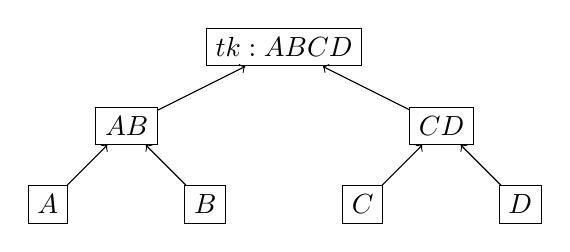
\begin{tikzpicture}[]
		\path (3, 3) node[rectangle, draw](root) {$ tk: ABCD $}
  		(1, 2) node[rectangle, draw] (ab) {$AB$}
  		(5, 2) node[rectangle, draw] (cd) {$CD$}
  		(0, 1) node[rectangle, draw] (a) {$A$}
  		(2, 1) node[rectangle, draw] (b) {$B$}
  		(4, 1) node[rectangle, draw] (c) {$C$}
  		(6, 1) node[rectangle, draw] (d) {$D$};

		\draw[->] (ab) -- (root);
		\draw[->] (cd) -- (root);
		\draw[->] (a) -- (ab);
		\draw[->] (b) -- (ab);
		\draw[->] (c) -- (cd);
		\draw[->] (d) -- (cd);
	\end{tikzpicture}
\end{frame}

\begin{frame}{Asynchronous Ratcheting Tree : ART — Cohn Gordon et al.~\cite{art}}
	\center
  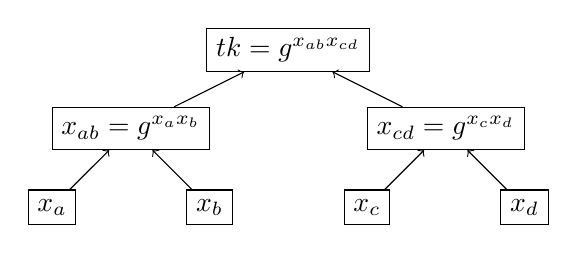
\begin{tikzpicture}[]
		\path (3, 3) node[rectangle, draw](root) {$ tk = g^{x_{ab} x_{cd}} $}
  		(1, 2) node[rectangle, draw] (ab) {$x_{ab} = g^{x_a x_b}$}
  		(5, 2) node[rectangle, draw] (cd) {$x_{cd} = g^{x_c x_d}$}
  		(0, 1) node[rectangle, draw] (a) {$x_a$}
  		(2, 1) node[rectangle, draw] (b) {$x_b$}
  		(4, 1) node[rectangle, draw] (c) {$x_c$}
  		(6, 1) node[rectangle, draw] (d) {$x_d$};

		\draw[->] (ab) -- (root);
		\draw[->] (cd) -- (root);
		\draw[->] (a) -- (ab);
		\draw[->] (b) -- (ab);
		\draw[->] (c) -- (cd);
		\draw[->] (d) -- (cd);
	\end{tikzpicture}

	\center
  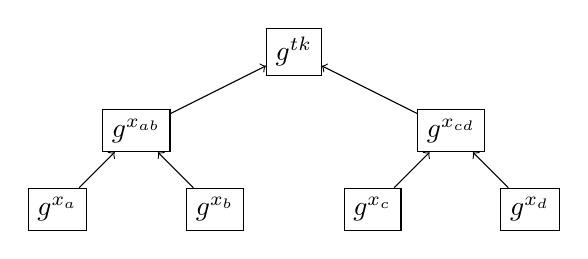
\begin{tikzpicture}[]
		\path (3, 3) node[rectangle, draw](root) {$ g^{tk} $}
  		(1, 2) node[rectangle, draw] (ab) {$g^{x_{ab}}$}
  		(5, 2) node[rectangle, draw] (cd) {$g^{x_{cd}}$}
  		(0, 1) node[rectangle, draw] (a) {$g^{x_a}$}
  		(2, 1) node[rectangle, draw] (b) {$g^{x_b}$}
  		(4, 1) node[rectangle, draw] (c) {$g^{x_c}$}
  		(6, 1) node[rectangle, draw] (d) {$g^{x_d}$};

		\draw[->] (ab) -- (root);
		\draw[->] (cd) -- (root);
		\draw[->] (a) -- (ab);
		\draw[->] (b) -- (ab);
		\draw[->] (c) -- (cd);
		\draw[->] (d) -- (cd);
	\end{tikzpicture}
\end{frame}

\begin{frame}{ART}
	\center
  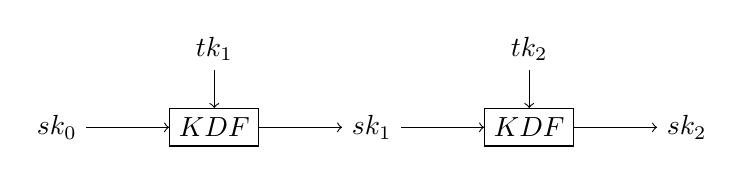
\begin{tikzpicture}[]
  	\path (0,0) node(sk0){$sk_0$} 
			(2, 1) node (tk0){$tk_1$}
  		(2, 0) node[rectangle, draw](kdf1){$KDF$}
  		(4, 0) node(sk1){$sk_1$}
			(6, 1) node (tk1){$tk_2$}
  		(6, 0) node[rectangle, draw](kdf2){$KDF$}
  		(8, 0) node(sk2){$sk_2$};

  	\draw[->](sk0) -- (kdf1);
		\draw[->](tk0) -- (kdf1);
		\draw[->](kdf1) -- (sk1);
  	\draw[->](sk1) -- (kdf2);
		\draw[->](tk1) -- (kdf2);
		\draw[->](kdf2) -- (sk2);
  \end{tikzpicture}

\end{frame}

\begin{frame}{ART : Send messages}
	\begin{block}{Send}
		\begin{itemize}
			\item Cypher with $sk$
			\item Broadcast
			\item Update Key
		\end{itemize}
	\end{block}

	\begin{block}{Update Key}
		\begin{itemize}
			\item Generate new $x, g^x$
			\item Broadcast the new public keys on the path
		\end{itemize}
	\end{block}
\end{frame}

\begin{frame}{ART : Update key}
	\center
  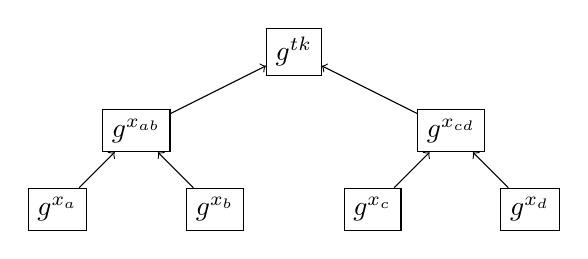
\begin{tikzpicture}[]
		\path (3, 3) node[rectangle, draw](root) {$ g^{tk} $}
  		(1, 2) node[rectangle, draw] (ab) {$g^{x_{ab}}$}
  		(5, 2) node[rectangle, draw] (cd) {$g^{x_{cd}}$}
  		(0, 1) node[rectangle, draw] (a) {$g^{x_a}$}
  		(2, 1) node[rectangle, draw] (b) {$g^{x_b}$}
  		(4, 1) node[rectangle, draw] (c) {$g^{x_c}$}
  		(6, 1) node[rectangle, draw] (d) {$g^{x_d}$};

		\draw[->] (ab) -- (root);
		\draw[->] (cd) -- (root);
		\draw[->] (a) -- (ab);
		\draw[->] (b) -- (ab);
		\draw[->] (c) -- (cd);
		\draw[->] (d) -- (cd);
	\end{tikzpicture}

  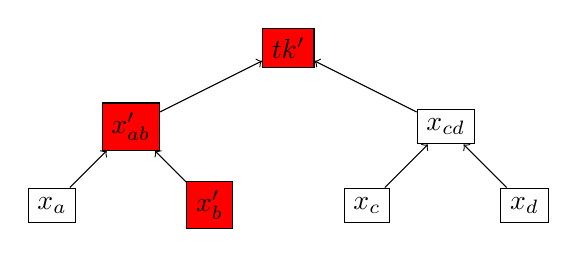
\begin{tikzpicture}[]
		\path (3, 3) node[rectangle, fill=red, draw](root) {$ tk' $}
  		(1, 2) node[rectangle, fill=red, draw] (ab) {$x_{ab}'$}
  		(5, 2) node[rectangle, draw] (cd) {$x_{cd}$}
  		(0, 1) node[rectangle, draw] (a) {$x_a$}
  		(2, 1) node[rectangle, fill=red, draw] (b) {$x_b'$}
  		(4, 1) node[rectangle, draw] (c) {$x_c$}
  		(6, 1) node[rectangle, draw] (d) {$x_d$};

		\draw[->] (ab) -- (root);
		\draw[->] (cd) -- (root);
		\draw[->] (a) -- (ab);
		\draw[->] (b) -- (ab);
		\draw[->] (c) -- (cd);
		\draw[->] (d) -- (cd);
	\end{tikzpicture}
\end{frame}

\begin{frame}{ART : Setup}
	\begin{block}{Building the tree}
  	\begin{itemize}
  		\item Get the signed public key of all participants
			\item Broadcast the public key of all participants
			\item Broadcast the tree topology
			\item Start the conversation
  	\end{itemize}
	\end{block}
\end{frame}

\begin{frame}{ART}
	\center
  	\begin{tabular}{c|cccc}
			 & mpOTR & GOTR & Signal & ART\\
			\hline
  		Authentification & \okay & \okay & \okay & \nope \\
  		\hline
  		Participants Coherence & \okay & \okay & \nope & \okay \\
  		Transcript Coherence & \okay & \okay & \nope & \nope \\
  		\hline
  		Message Repudiation & \okay & \okay & \okay & \okay \\
  		Participation Repudiation & \okay & \okay & \okay & \okay \\
  		\hline
  		Dynamic Groups & \nope & \okay & \okay & \okay\\
  		\hline
  		Forward Secrecy & \nope & \sortof & \sortof & \okay \\
  		Backward Secrecy & \nope & \sortof & \okay & \okay\\
  		Non-Transitivity of Messages & \nope & \okay & \okay & \okay \\
  		\hline
  		Asynchrone & \sortof & \nope & \okay & \okay 
    \end{tabular}
\end{frame}

\section{And now ?}
\begin{frame}{ART 2.0 : Authenticated}
	\begin{block}{Main ideas}
		\begin{itemize}
			\item Unique public keys
			\item Dynamic keys ! 
		\end{itemize}		
	\end{block}
	\pause
	\begin{block}{Dynamic keys}
		\begin{itemize}
			\item $(x, g^x) \ra (x', g^{x'})$
			\item $f, h$ st. $g^{f(x)} = h(g^x)$
		\end{itemize}
	\end{block}
\end{frame}

\begin{frame}{ART : Dynamic Diffie-Hellman}
	\begin{block}{One solution}
		\begin{itemize}
			\item $f : x \ra 2x$
			\item $h : y \ra y^2$
			\item $g^{2x} = (g^x)^2$
		\end{itemize}
	\end{block}
	\pause
	\begin{block}{Adapt the solution}
		\begin{itemize}
			\item $f : x \ra tk\cdot x$
			\item $h : y \ra y^{tk}$
			\item $g^{tk\cdot x} = (g^x)^{tk}$
		\end{itemize}
	\end{block}
\end{frame}

\begin{frame}{ART : Not a perfect solution}
	\begin{block}{Problems}
		\begin{itemize}
			\item The first step ?
			\item Can't build a credible transcript
			\item Break the crypto ?
		\end{itemize}
	\end{block}
	\center
	Working on it.
\end{frame}
\section*{Thanks ! Questions ?}

\section*{Bibliography}
\begin{frame}
  \begin{small}

    \bibliographystyle{abbrv}
    \bibliography{slides}
	\end{small}
\end{frame}

\end{document}
